\chapter{方案部署及其效果}
\label{cha:experiment}
本章的主要内容为部署防御方案并验证方案有效性。在真实SDN网络中部署防御方案之后,使用不同形式的LDoS攻击对方案进行测试,探测方案的有效性与开销。

\section{实验准备}
\label{chap5:setup}
本文在真实SDN网络中部署防御系统。防御系统使用的SDN控制器为Floodlight控制器。部署了防御系统的控制器被部署在一个服务器上,该服务器的配置为Intel Xeon Quad-Core CPU E5504和4GB的RAM。在系统中我们使用了OpenFlow商业硬件交换机(EdgeCore AS4610-54T)作为真实SDN网络使用的硬件交换机。硬件交换机的端口转发速率最高能够可达到1Gbps,本文将最大转发速率标记为$R_m$。为了验证系统有效性,本文使用C代码生成不同$T$与$L$的LDoS攻击。并且使用Python代码完成分布式LDoS攻击的部署。

图\ref{fig:topology}展示了实验使用的SDN网络拓扑图。它有7个主机和3个OpenFlow硬件交换机组成。其中2个主机为攻击主机,5个主机为正常的主机。在实验中,$h_1$发送正常流量作为背景流量并由$h_5$接收,$h_3$与$h_6$之间建立TCP连接。$h_2$和$h_4$被设置为LDoS攻击的发送端,由$h_7$接收他们发送的LDoS攻击流量。对于攻击者$h_2$和$h_4$的不同配置可以得到单一攻击源的LDoS攻击,也可以得到分布式LDoS攻击。

%对于这个网络,LDoS攻击流的目的是完全占用$S_2$与$S_3$之间连接的带宽致使$S_2$的队列被拥塞造成$h_1$

\begin{figure}
    \centering
    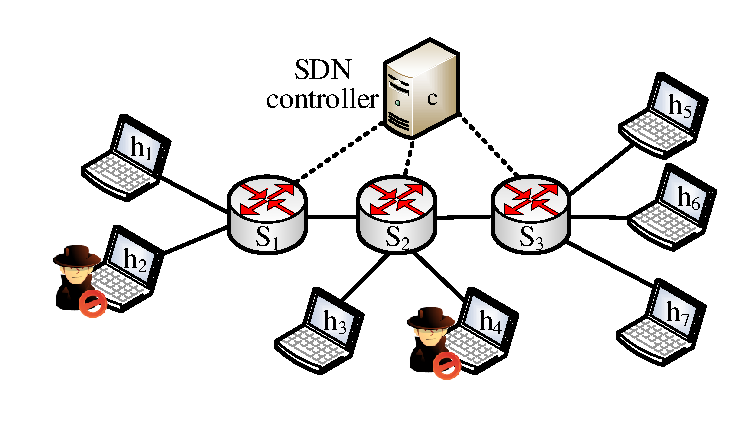
\includegraphics[scale=1]{topology}
    \caption{实验使用拓扑图}
    \label{fig:topology}
\end{figure}


\section{基于带宽保障的方案}
\label{chap5:bandwidth-reserve-solution}

这个部分通过对部署了基于带宽保障的方案的系统的有效性和开销进行评估,分析该方案的效果。在不同保留带宽的条件下,测试TCP流的吞吐量已验证有效性。在部署防御系统的情况下通过生成不同$T$的LDoS攻击测试系统的开销。

\begin{figure}
    \begin{subfigure}{.49\textwidth}
        \centering
        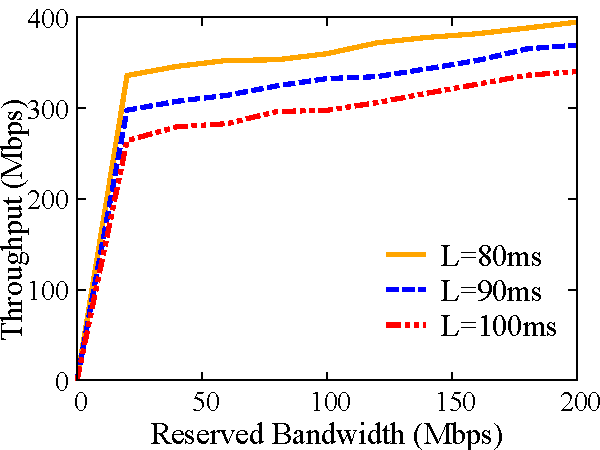
\includegraphics[scale=0.7]{reserved-bandwidth}
        \caption{单攻击源}
        \label{fig:reserved-bandwidth-single}
    \end{subfigure}
    \begin{subfigure}{.49\textwidth}
        \centering
        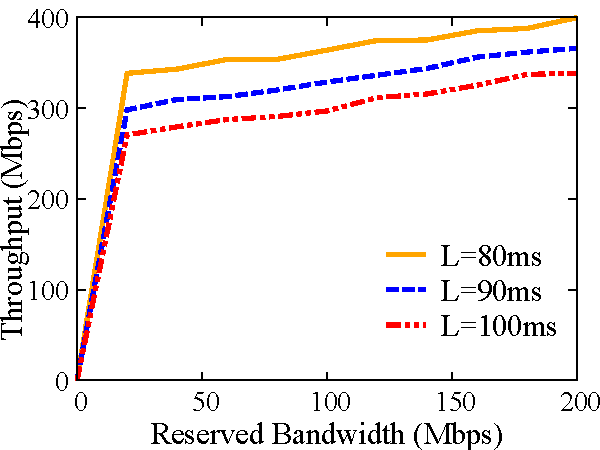
\includegraphics[scale=0.7]{reserved-bandwidth1}
        \caption{分布式方案一}
        \label{fig:reserved-bandwidth-2h-mod1}
    \end{subfigure}

    \begin{subfigure}{.49\textwidth}
        \centering
        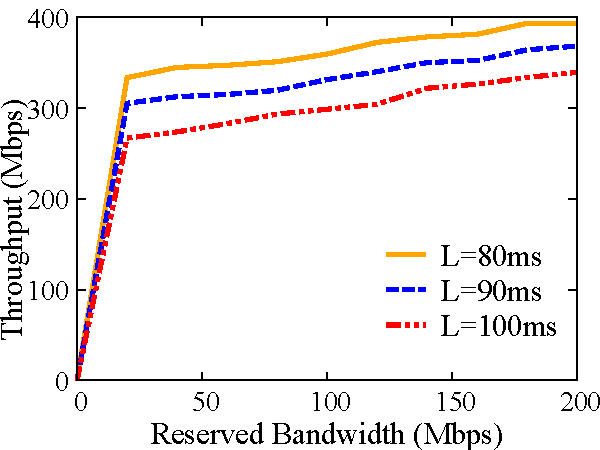
\includegraphics[scale=0.7]{reserved-bandwidth2}
        \caption{分布式方案二}
        \label{fig:reserved-bandwidth-2h-mod2}
    \end{subfigure}
    \begin{subfigure}{.49\textwidth}
        \centering
        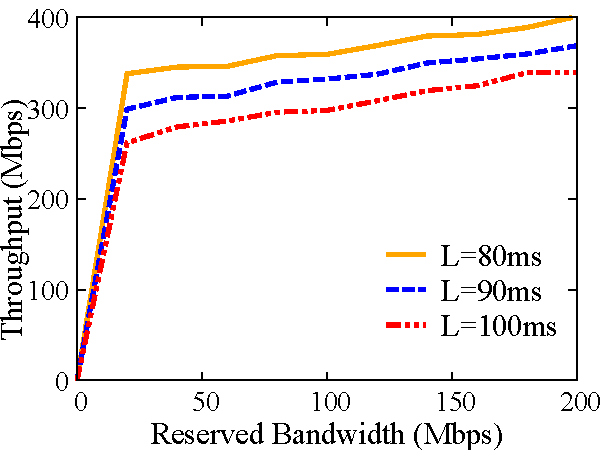
\includegraphics[scale=0.7]{reserved-bandwidth3}
        \caption{分布式方案三}
        \label{fig:reserved-bandwidth-2h-mod3}
    \end{subfigure}


    \caption{不同LDoS攻击下,TCP流的聚合吞吐量平均值}
    \label{fig:reserved-bandwidth-all}
\end{figure}

为了验证系统有效性,在LDoS攻击存在的时候,本文测试了TCP流的聚合吞吐量。在系统生成了100个TCP流,而且这些流经过共同的端口。攻击主机以单攻击源和分布式方案等四种方式发送LDoS攻击流(在$T$为210毫秒,$R$为1Gbps),这些流也经过改端口,并注入背景流量。在设置Meter规则的粒度为RTT级别之后,将非TCP流的流表规则与相应的Meter规则绑定,通过限制非TCP流的速率保留了TCP的流带宽。接下来,在LDoS的攻击下,改变保留带宽的大小的同时测试TCP流的聚合吞吐量。实验测试了保留带宽由0至200Mbps的条件下,30秒内TCP流的聚合吞吐量平均值。实验测试了不同$L$的LDoS以验证方案的稳定性。图\ref{fig:reserved-bandwidth-single}为在单攻击源的LDoS攻击下,使用带宽保障方案之后的TCP流的聚合吞吐量平均值。可以看出,为TCP流保留的带宽越多,则TCP流的吞吐量越大。在保留带宽为0,即没有部署防御系统的时候,TCP流的聚合吞吐量平均值近乎为0,因为LDoS攻击迫使TCP流进入超时重传状态,仅发送少量的探测数据包。当保留带宽为20Mbps时,TCP流带宽上升至250Mbps,因为TCP流有保留带宽,不会因为丢包而进入超时重传窗台,吞吐量平均值上升。在保留带宽增大的情况下,吞吐量平均值上升缓慢上升是因为LDoS攻击流占用的部分带宽被TCP流使用。

图\ref{fig:reserved-bandwidth-2h-mod1}为分布式方案一的LDoS攻击下,使用带宽保障方案之后的TCP流的聚合吞吐量平均值。图\ref{fig:reserved-bandwidth-2h-mod2}为分布式方案二的LDoS攻击下,使用带宽保障方案之后的TCP流的聚合吞吐量平均值。图\ref{fig:reserved-bandwidth-2h-mod3}为分布式方案三的LDoS攻击下,使用带宽保障方案之后的TCP流的聚合吞吐量平均值。从这三个图中,可以看出,分布式的LDoS攻击也会被Meter规则限制峰值速率,因为保留了TCP流的部分带宽,无法强迫TCP流进入超时重传状态。



\begin{figure}
    \begin{subfigure}{.49\textwidth}
        \centering
        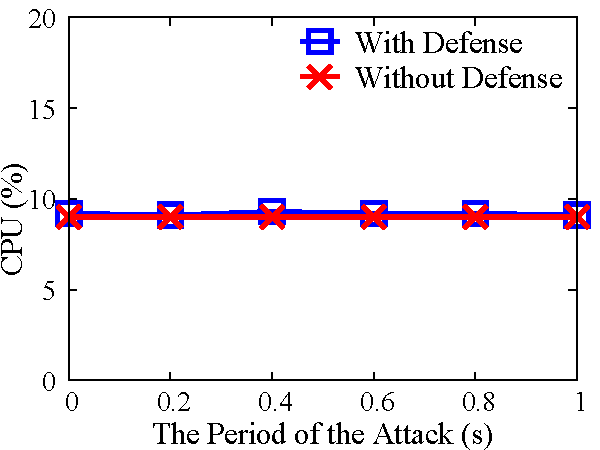
\includegraphics[scale=0.7]{reserved-utilizaition}
        \caption{单攻击源}
        \label{fig:reserved-CPU-single}
    \end{subfigure}
    \begin{subfigure}{.49\textwidth}
        \centering
        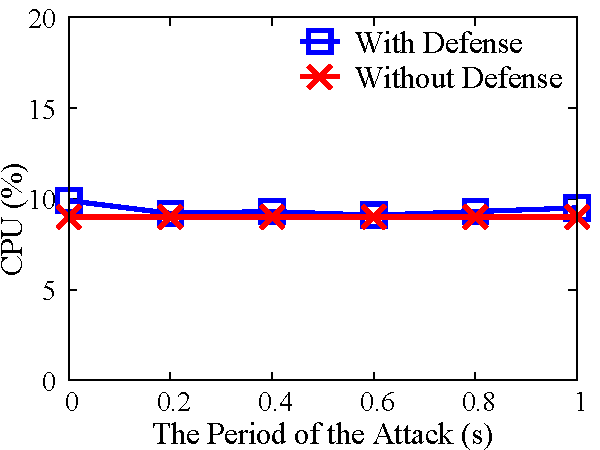
\includegraphics[scale=0.7]{reserved-utilizaition1}
        \caption{分布式方案一}
        \label{fig:reserved-CPU-2h-mod1}
    \end{subfigure}

    \begin{subfigure}{.49\textwidth}
        \centering
        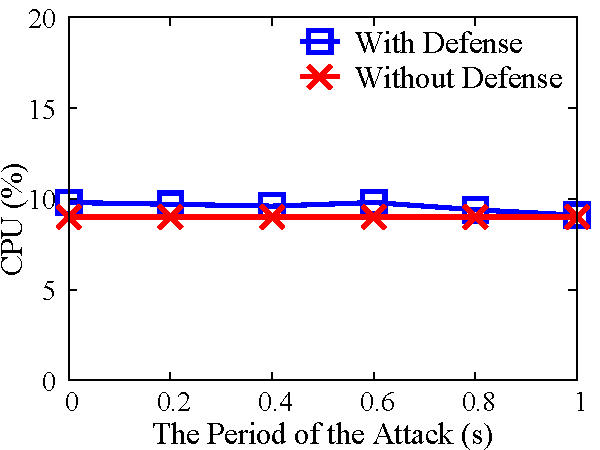
\includegraphics[scale=0.7]{reserved-utilizaition2}
        \caption{分布式方案二}
        \label{fig:reserved-CPU-2h-mod2}
    \end{subfigure}
    \begin{subfigure}{.49\textwidth}
        \centering
        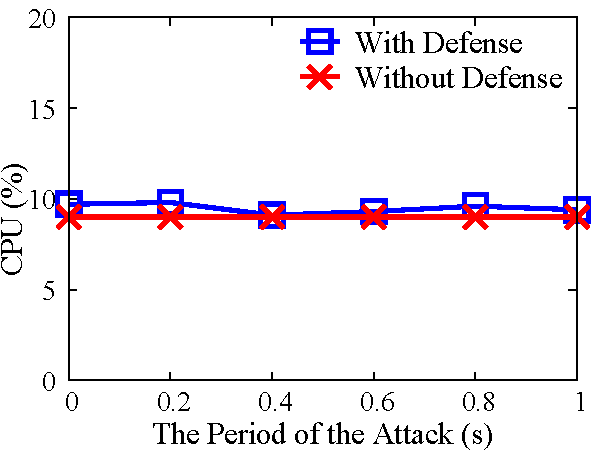
\includegraphics[scale=0.7]{reserved-utilizaition3}
        \caption{分布式方案三}
        \label{fig:reserved-CPU-2h-mod3}
    \end{subfigure}


    \caption{CPU使用率}
    \label{fig:reserved-CPU-all}
\end{figure}


在控制器上部署了基于带宽保障的防御方案之后,通过观察控制器的CPU使用率,分析系统开销。实验中,测试了$T$从0.1秒上升至1秒的LDoS攻击流。从图\ref{fig:reserved-CPU-all}可以看出,不管面对单攻击源还是分布式的LDoS攻击,引入的系统额外开销都低于1\%。由于防御方案没有对数据流做深入的分析,而只是在确认数据流不是TCP流时,将该流的流表规则与Meter规则绑定以限制该流的上限速率,所以,基于带宽保障的方案虽然开销极小,但是依然能够保证TCP流不进入超时重传状态。


%\subsection{系统开销}


\section{基于动态周期性检测的防御方案}
\label{chap5:exp-period-detection}
在系统部署了基于动态周期性检测的方案之后,本文通过对检测精确度和方案的开销对方案进行全方位的讨论和分析,对方案的有效性进行评价。

\subsection{精确度分析}
\label{chap5:accuracy}
这个部分主要分析基于动态周期性检测的防御方案的各个模块的准确性和稳定性。首先,本文对异常检测模块成功检测到端口异常的成功率做实验进行分析。然后,本文计算了攻击定位模块推断出的LDoS攻击周期与真正的LDoS周期之间的误差。接下来,本文通过实验获得了经过受影响端口与经过端口流量的平均欧式距离的概率密度函数(Probability Density Function,PDF),并在此基础上,找到了用于判断攻击流的阈值。最后,本文探索了平均欧式方法判断攻击流的准确度。

异常检测模块在异常端口处检测到可能的LDoS攻击时才会激活攻击定位模块对异常端口进行进一步的分析,因此,该模块在LDoS攻击存在的情况下检测到端口吞吐量异常的成功率直接关键到LDoS攻击能否被系统检测,因此,本文对异常检测模块的参数$\alpha$和$M$进行了探讨。



% alpha,M两个参数进行分析讨论,出图,(1-2页)

% alpha和LDoS识别率,M作为稳定参数,多次取值,准确识别LDoS的图

% alpha和误判率,M作为稳定参数,多次取值,正常流判断为LDoS流


攻击定位模块的第一步是对序列进行二值化,本文将阈值$\beta$设为0.8。接下来,本文通过对异常端口的计数器获取的数据推测LDoS攻击的周期。在获得二值化序列之后,本文对该序列进行周期性的推测。如果在异常的端口处存在LDoS攻击流,则推断出的序列周期将会是一个正数。但是,如果端口不存在LDoS攻击流,则推断出的序列周期将会为0。为了获得攻击定位模块推断的周期准确度,本文比较通过序列推断出的周期与LDoS攻击流的真实周期,得到了推断的周期误差。

\begin{figure}
    \begin{subfigure}{.49\textwidth}
        \centering
        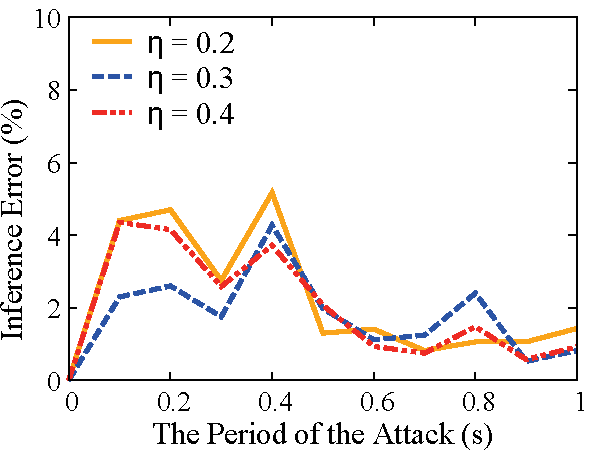
\includegraphics[scale=0.7]{period}
        \caption{单攻击源}
        \label{fig:period-single}
    \end{subfigure}
    \begin{subfigure}{.49\textwidth}
        \centering
        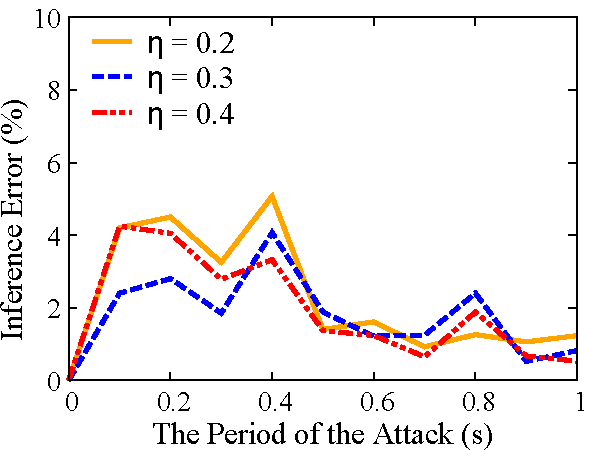
\includegraphics[scale=0.7]{period1}
        \caption{分布式方案一}
        \label{fig:period-2h-mod1}
    \end{subfigure}

    \begin{subfigure}{.49\textwidth}
        \centering
        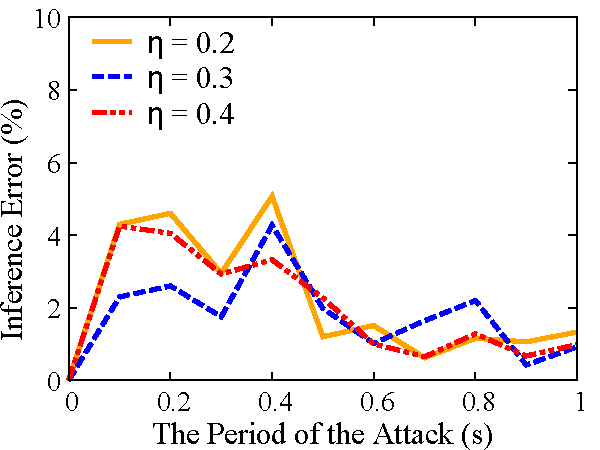
\includegraphics[scale=0.7]{period2}
        \caption{分布式方案二}
        \label{fig:period-2h-mod2}
    \end{subfigure}
    \begin{subfigure}{.49\textwidth}
        \centering
        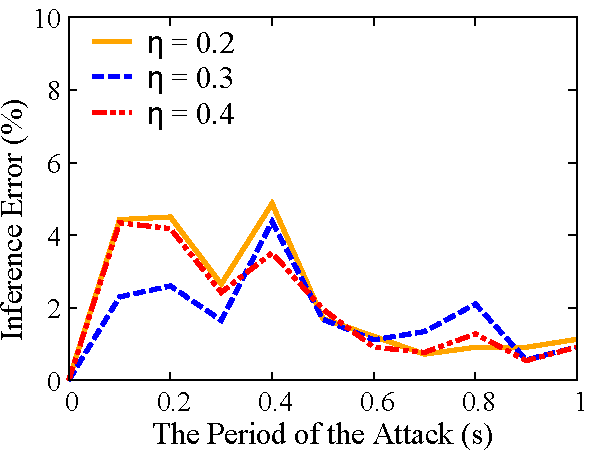
\includegraphics[scale=0.7]{period3}
        \caption{分布式方案三}
        \label{fig:period-2h-mod3}
    \end{subfigure}


    \caption{不同LDoS攻击的周期推断误差}
    \label{fig:period-all}
\end{figure}


实验对单攻击源和三种分布式方案进行了测试,推断不同LDoS攻击的误差。使用算法\ref{alg:port_locate}来预测LDoS攻击的周期。实验中,我们将LDoS攻击的突发速率$R$置为1Gbps。对于算法的参数,考虑系统的带宽和识别率保证,本文设定$T_e$为0.005,$T_i$为0.64,$\epsilon$ = 0.01。为了查看算法对LDoS攻击周期的适应性,在LDoS攻击的周期从0.1上升至1s的情况下,使用攻击定位模块对不同$\eta$值的LDoS攻击的周期进行预测。除此之外,还使用洪泛攻击测试算法。每次使用5秒获取端口的数据进行测试。首先考虑单攻击源LDoS攻击。在不同LDoS攻击的周期下,攻击定位模块推断的周期与真实LDoS攻击的周期的相对误差。实验结果如图\ref{fig:period-single}所示。结果表示,攻击检测模块能够确认异常端口上的LDoS攻击,同时,推测出来的周期也存在一定的误差,但是,推断出的相对误差最多不超过6\%。LDoS攻击不存在(洪泛攻击)的情况下,由于洪泛攻击没有周期,而推断出的周期为0,因此,在0点处,误差为0。在大多数情况下,在LDoS攻击的周期值比较小的时候,相对误差会比较大。攻击检测模块的绝对误差在0至30毫秒之间,随着算法的周期不断变大,攻击检测模块的相对误差也相应的减小。

图\ref{fig:period-2h-mod1}攻击定位模块预测分布式方案一的LDoS攻击周期的误差。与单攻击源相似,都能够确认LDoS攻击的周期性,而且推断的误差基本都低于5\%,$\eta$值的变化对于分布式方案一周期的推断影响不大,这样的误差对于系统推断端口吞吐量的周期性是可以接受的。

图\ref{fig:period-2h-mod2}攻击定位模块预测分布式方案二的LDoS攻击周期的误差。通过都能够确认LDoS攻击的周期性,而且推断的误差基本都集中在3\%。$\eta$值的变化不影响攻击定位模块确认端口吞吐量的周期性。而且,推断出的周期误差是可以接受的。

图\ref{fig:period-2h-mod3}攻击定位模块预测分布式方案三的LDoS攻击周期的误差。攻击定位模块在异常端口处推断LDoS的误差不高于6\%。异常端口是否受到LDoS攻击的影响都可以确认,因为端口流量的周期性是可以被攻击定位模块确认的。

综上所述,攻击定位模块能够获得异常端口流量的周期性,从而确认LDoS攻击。不管是单攻击源还是分布式的LDoS攻击能够被攻击定位模块检测出。而且,误差值都在可接受的范围,不影响LDoS攻击的周期性确认。$\eta$值的大小不影响异常端口处对于LDoS攻击的判断。通过这次实验也获得了相应的$T_s$。攻击定位模块在确认了LDoS攻击在异常端口存在之后,使用了$T_s$作为采样间隔获取流表规则上的计数器数据用以对识别攻击流。

在确认端口受LDoS攻击影响之后,控制器以$T_s$的采样间隔同时获取受影响端口序列与经过该端口的流的信息,在通过二值化之后对二值化流量做进一步分析。在LDoS攻击的$T$设为1秒,$L$设为0.2秒的时候,控制器以$T_s$为0.1s获取流表规则计数器上的数据,则可以获得受影响端口、正常数据流和LDoS攻击流的吞吐量二值化序列。实验测试了单攻击源和分布式LDo攻击的情况。首先是单攻击源的LDoS攻击。如图\ref{fig:binary-sequence-single}所示,三者的吞吐量二值化序列的形状是完全不同的,受影响端口的二值化序列的形状与LDoS攻击流的二值化序列更加相近,而背景流量的形状则与受影响端口的二值化序列不相似。在LDoS突发出现的时候,即图中LDoS攻击的二值化吞吐量值为1的时候,受影响端口的二值化吞吐量也为1,此时,背景流量的二值化吞吐量为0,因为,在LDoS攻击的突发时间里的情况下,交换机转发的背景流量低于没有LDoS攻击时的最高速率,在二值化的时候把该时刻的值置为0。LDoS攻击的二值化序列周期$T_b$为10。也存在部分受影响端口的二值化吞吐量值为1,但没有LDoS攻击流,这是背景流经过受影响端口造成的。在LDoS攻击存在的情况下,受影响端口统计的吞吐量序列最大值$S_m$即为$R_m$,因此,受影响端口统计的吞吐量序列中流量的速率在LDoS攻击不存在的情况下基本低于$\beta * S_m$。受影响端口在LDoS攻击不存在的情况下的二值化吞吐量基本为0。

以分布式方案一的方式生成LDoS攻击流。控制器通过获取受影响端口、一条正常数据流和一条LDoS攻击流的吞吐量并对其二值化,得到二值化序列,如图\ref{fig:binary-sequence-2h-mod1}所示。可以看出,LDoS攻击流的$T_b$为20,相较于单攻击源,周期更大。在LDoS攻击流的二值化吞吐量为1的时候,受影响端口的二值化吞吐量为1,正常流的二值化吞吐量为0,这说明,该LDoS攻击流突发时占用了受影响端口的所有带宽。但是,也存在受影响端口的二值化吞吐量为1的时候,攻击流的二值化吞吐量为0,大部分这种情况是另一条LDoS攻击流造成的,还有一部分是正常流造成的。相较于分布式方案一的二值化吞吐量,单攻击源的LDoS攻击流的二值化吞吐量与受影响端口的二值化吞吐量相似程度更高,因为分布式方案一使每个LDoS攻击流的周期变成了单攻击源的两倍,因此,隐蔽性更强。


以分布式方案二的方式生成LDoS攻击流。控制器通过获取受影响端口、一条正常数据流和一条LDoS攻击流的吞吐量并对其二值化,得到二值化序列,如图\ref{fig:binary-sequence-2h-mod2}所示。可以看出,LDoS攻击流的$T_b$为10,与单攻击源周期相同。在LDoS攻击流的二值化吞吐量为1的时候,受影响端口的二值化吞吐量为1,正常流的二值化吞吐量为0,两条LDoS攻击流突发时占用了受影响端口的所有带宽。但是,也存在受影响端口的二值化吞吐量为1的时候,攻击流的二值化吞吐量为0,这是正常流经过受影响端口的结果。分布式方案二与单攻击源的LDOS攻击的二值化序列相似,因为,分布式方案二只改变了每个LDoS攻击流的突发速率,未改变LDoS攻击流的持续时间长度。

以分布式方案三的方式生成LDoS攻击流。控制器通过获取受影响端口、一条正常数据流和一条LDoS攻击流的吞吐量并对其二值化,得到二值化序列,如图\ref{fig:binary-sequence-2h-mod3}所示。可以看出,LDoS攻击流的$T_b$为20,相较于单攻击源,周期更大。在LDoS攻击流的二值化吞吐量为1的时候,受影响端口的二值化吞吐量为1,正常流的二值化吞吐量为0。不过,有时候,该攻击流的二值化吞吐量为0,受影响端口的二值化吞吐量为1,另一条LDoS攻击与正常流经过端口造成了这样的结果。对于受影响端口的二值化吞吐量而言,值为1都是LDoS攻击流量经过端口的的结果。分布式方案三的隐蔽效果也比单攻击源更好。

综上所述,四种LDoS攻击的二值化序列如图\ref{fig:binary-sequence-all}所示。分布式方案一与分布式方案三的二值化序列与受影响端口的二值化序列相似度要低一些,因为两种方案改变了单个LDoS攻击流的突发持续时间。而单攻击源与分布式方案二的LDoS攻击流的二值化序列与受影响端口的二值化序列相似度要更高,也更易于识别。


\begin{figure}
    \begin{subfigure}{.49\textwidth}
        \centering
        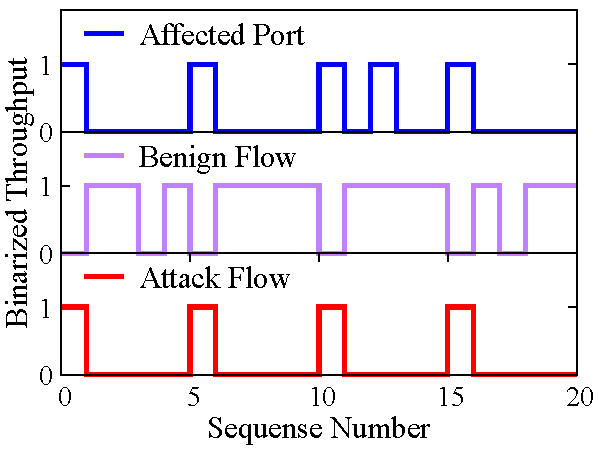
\includegraphics[scale=0.7]{binary-sequence}
        \caption{单攻击源}
        \label{fig:binary-sequence-single}
    \end{subfigure}
    \begin{subfigure}{.49\textwidth}
        \centering
        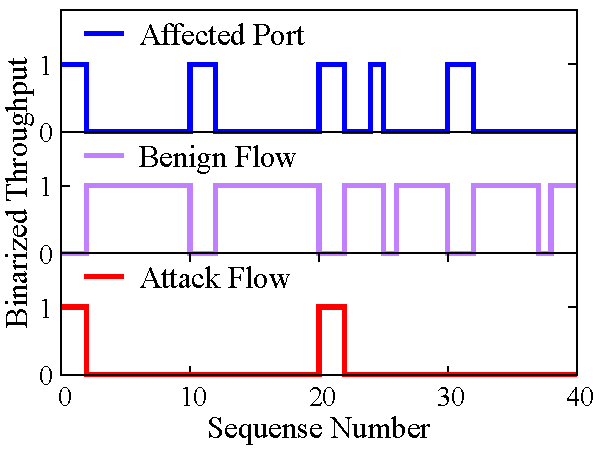
\includegraphics[scale=0.7]{binary-sequence1}
        \caption{分布式方案一}
        \label{fig:binary-sequence-2h-mod1}
    \end{subfigure}

    \begin{subfigure}{.49\textwidth}
        \centering
        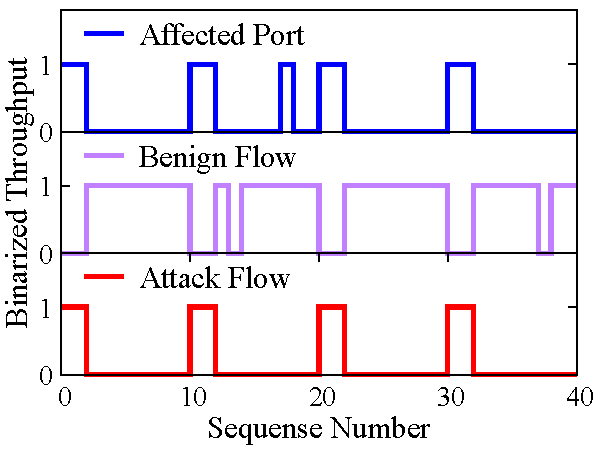
\includegraphics[scale=0.7]{binary-sequence2}
        \caption{分布式方案二}
        \label{fig:binary-sequence-2h-mod2}
    \end{subfigure}
    \begin{subfigure}{.49\textwidth}
        \centering
        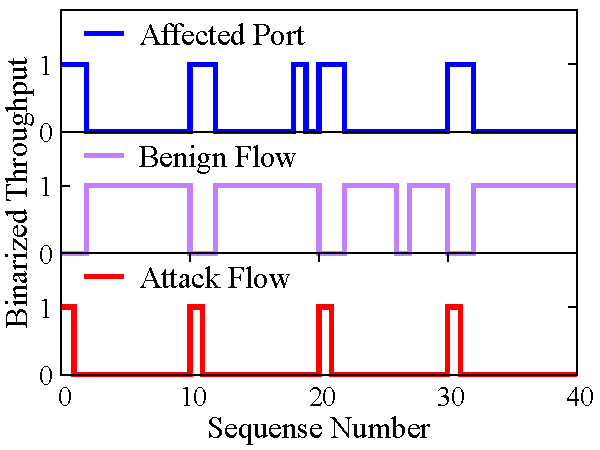
\includegraphics[scale=0.7]{binary-sequence3}
        \caption{分布式方案三}
        \label{fig:binary-sequence-2h-mod3}
    \end{subfigure}


    \caption{LDoS存在时,二值化吞吐量序列}
    \label{fig:binary-sequence-all}
\end{figure}

% \begin{figure}
%     \centering
%     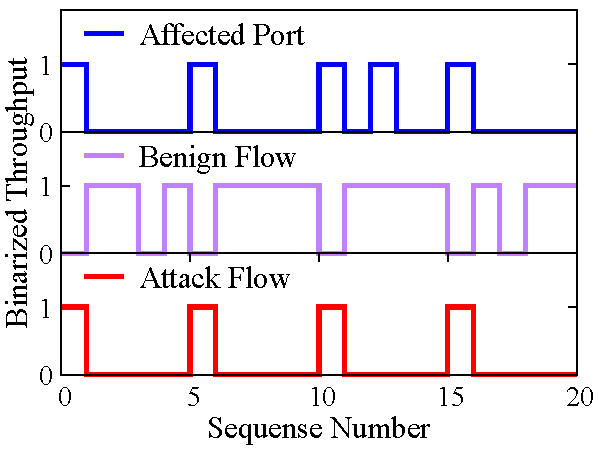
\includegraphics[scale=1.3]{binary-sequence}
%     \caption{二值化吞吐量序列}
%     \label{fig:binary-sequence}
% \end{figure}



为了获得合适的阈值$\gamma$来识别攻击流,受影响端口的二值化序列与经过该端口的数据流的平均欧式距离的概率密度函数是必须的,但是一个攻击源与多个攻击源的情况不同,因此,需要多次试验来分析不同的情况下。LDoS攻击流平均欧氏距离与正常数据流的平均欧氏距离是完全不同的。在经过了二值化之后,LDoS攻击流的二值化序列与受影响端口统计的二值化序列的平均欧式距离比正常流量小很多,因此,找到合适的阈值$\gamma$,就可以识别攻击流。首先,考虑验证系统对于大部分情况的适应性,只用一个固定的$T$是不足够的,所以,LDoS攻击的$T$随机从0.8至1.5之前取值,因为LDoS攻击的$T$取值过大会是TCP流无法进入超时重传状态。接下来,考虑到$L$的取值不应过小或者过大,设置LDoS攻击的突发长度$L$从0.1至0.4之间随机取值。如果$L$太小,则无法造成TCP流丢包,则无法达到LDoS攻击的效果。但是,如果$L$的取值过大,则平均速率会很高,容易被洪泛服务拒绝攻击的检测方式检测到。最后,考虑交换机最大转发速率为1Gbps,所以,LDoS攻击的突发速率$R$设为1Gbps已经是能够达到的最大速率了,如果突发速率更高则可能造成LDoS攻击自身丢包过多,反而容易被检测到。考虑到需要有背景流量作为良性的流量干扰防御系统以验证攻击定位模块的有效性,$h_1$生成了100条良性流作为背景流量发送给$h_5$。

本文先分析一个攻击源生成LDoS攻击的情况。以$h_2$作为攻击源发送LDoS攻击流,$h_4$不发送攻击流量。经过多次试验,获得图\ref{fig:PDF-single}作为单攻击源的概率密度函数。可以看到,LDoS攻击流的二值化序列与受影响端口的二值化序列的平均欧式距离的主要分布在0.2与0.4之间,平均值为0.3。而正常流的二值化序列与受影响端口的二值化序列的平均欧式距离的主要分布在0.44至0.84之间,平均值为0.64。绝大部分情况下,LDoS攻击流的二值化序列与受影响端口的二值化序列的平均欧式距离比正常流的二值化序列与受影响端口的二值化序列的平均欧式距离小。因为在LDoS攻击突发存在的情况下,端口转发的主要流量为LDoS攻击。而没有LDoS攻击攻击存在的时候,正常流公平竞争带宽,因此,速率更高,在突发不存在的时候,二值化吞吐量值为1,受影响端口的二值化序列为0,刚好相反,因此平均欧式距离更大。从图\ref{fig:PDF-single}中可以看到一个清晰的区分点,即$MED$为0.42。该点可以作为识别单攻击源中LDoS攻击流的阈值。


\begin{figure}
    \begin{subfigure}{.49\textwidth}
        \centering
        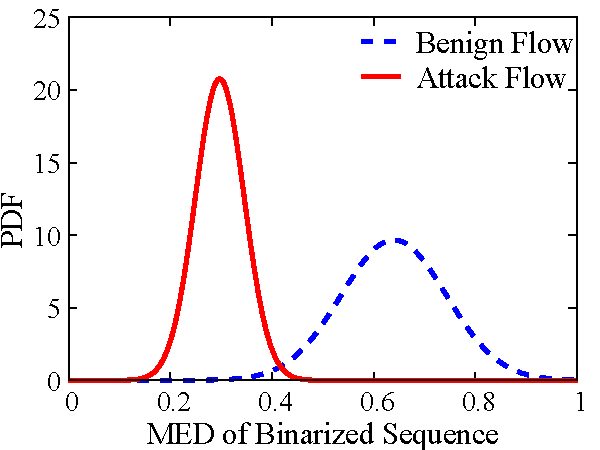
\includegraphics[scale=0.7]{distribution}
        \caption{单攻击源}
        \label{fig:PDF-single}
    \end{subfigure}
    \begin{subfigure}{.49\textwidth}
        \centering
        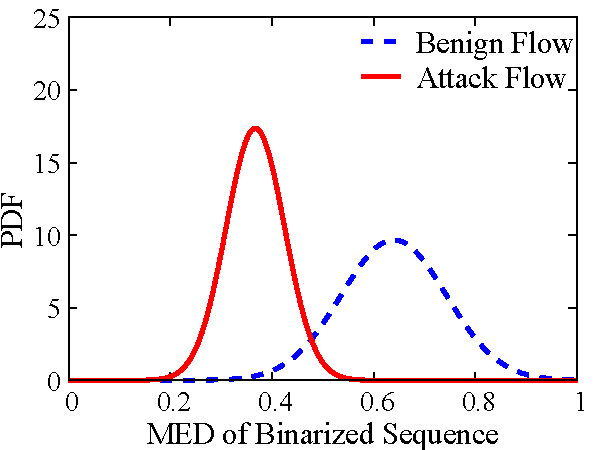
\includegraphics[scale=0.7]{distribution1}
        \caption{分布式方案一}
        \label{fig:PDF-2h-mod1}
    \end{subfigure}

    \begin{subfigure}{.49\textwidth}
        \centering
        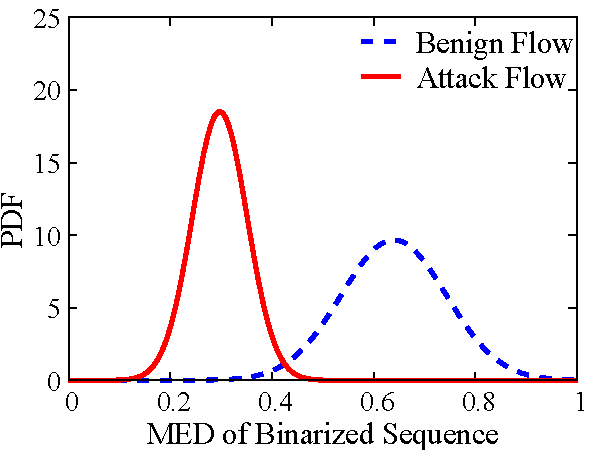
\includegraphics[scale=0.7]{distribution2}
        \caption{分布式方案二}
        \label{fig:PDF-2h-mod2}
    \end{subfigure}
    \begin{subfigure}{.49\textwidth}
        \centering
        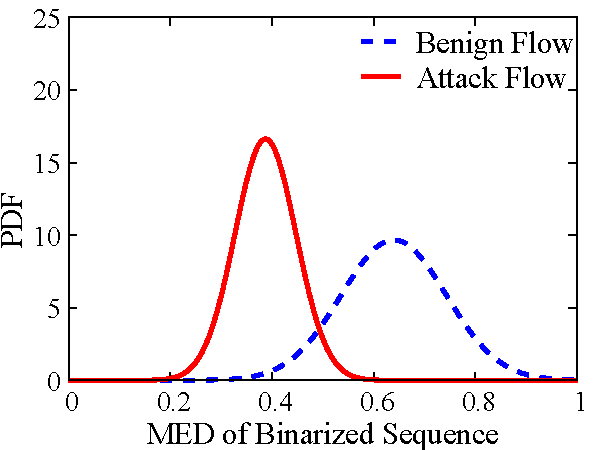
\includegraphics[scale=0.7]{distribution3}
        \caption{分布式方案三}
        \label{fig:PDF-2h-mod3}
    \end{subfigure}


    \caption{LDoS攻击流的平均欧式距离的概率密度函数}
    \label{fig:PDF-all}
\end{figure}



% \begin{figure}
%     \begin{minipage}[t]{0.49\linewidth}
%         \centering
%         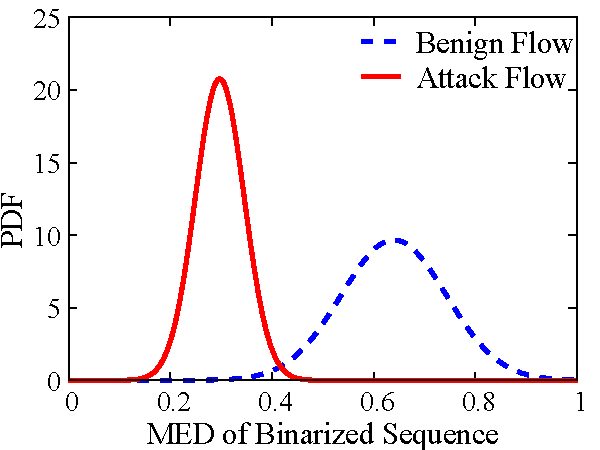
\includegraphics[scale=0.7]{distribution}
%         \caption{\small{单攻击源的平均欧式距离的PDF}}
%         \label{fig:PDF-single}
%     \end{minipage}
%     \begin{minipage}[t]{0.49\linewidth}
%         \centering
%         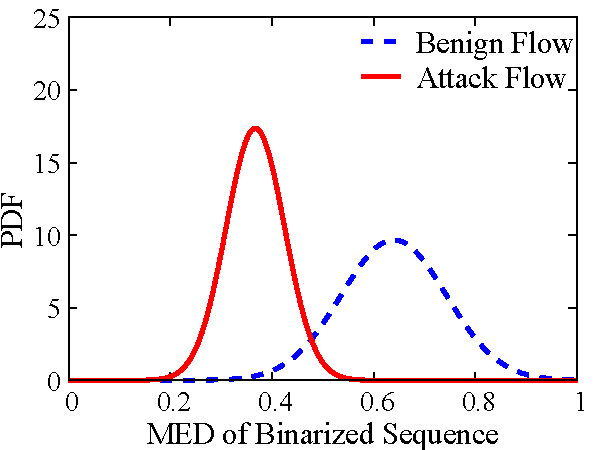
\includegraphics[scale=0.7]{distribution1}
%         \caption{\small{分布式方案一平均欧式距离的PDF}}
%         \label{fig:PDF-2h-mod1}
%     \end{minipage}

%     \begin{minipage}[t]{0.49\linewidth}
%         \centering
%         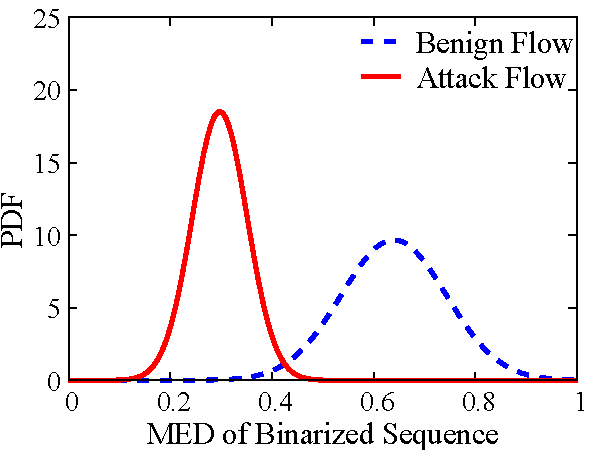
\includegraphics[scale=0.7]{distribution2}
%         \caption{\small{分布式方案二平均欧式距离的PDF}}
%         \label{fig:PDF-2h-mod2}
%     \end{minipage}
%         \begin{minipage}[t]{0.49\linewidth}
%         \centering
%         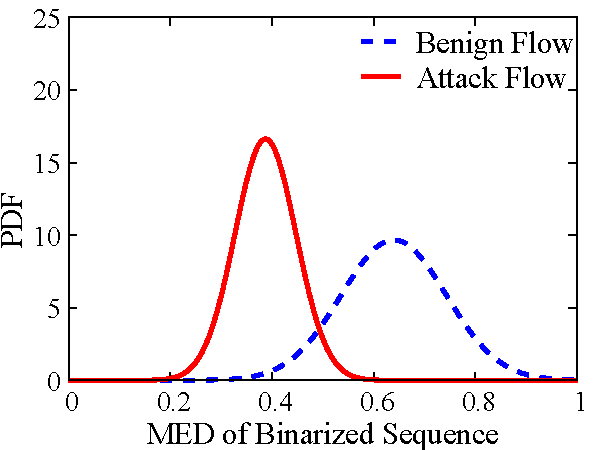
\includegraphics[scale=0.7]{distribution3}
%         \caption{\small{分布式方案三平均欧式距离的PDF}}
%         \label{fig:PDF-2h-mod3}
%     \end{minipage}
% \end{figure}

在获得单攻击源的平均欧式距离的概率分布函数之后,可以确认使用平均欧氏距离的方法确实可以区分攻击流与正常流。接下来,对多攻击源分布式LDoS攻击进行区分,因此,以$h_2$和$h_4$同时作为攻击源发送LDoS攻击流,分布式LDoS攻击的三种方案产生流量,获得相应的平均欧式距离的概率密度函数。两主机以分布式方案一的方式产生LDoS攻击的流量,获得图\ref{fig:PDF-2h-mod1}。从图中可看出,与单攻击源不同,LDoS攻击流的二值化序列与受影响端口的二值化序列的平均欧式距离的分布发生了变化,主要分布在0.24至0.48,平均值为0.36,而正常流的二值化序列与受影响端口的二值化序列的平均欧式距离的主要分布在0.45至0.85之间,平均值为0.65。方案一平均欧式距离的概率分布函数平均值相较于单攻击源的情况差别较大。因为在受影响端口处统计的突发包括了两个主机的突发流量,每个$T$内都包含一个突发。而使用流表规则统计的数据只包含一个流的数据,在$2T$内检测到一次突发。因此,计算出的平均欧式距离统计的平均值相较于单攻击源的平均欧式距离统计的平均值更大。因此,对于方案一而言,最佳的区分点为0.47。

当两个主机以分布式方案二的方式产生LDoS攻击的流量,获得图\ref{fig:PDF-2h-mod2}。从图中可看出,LDoS攻击流的二值化序列与受影响端口的二值化序列的平均欧式距离的分布与单攻击源相似,主要集中在0.21至0.41之间,平均值为0.31。正常流的二值化序列与受影响端口的二值化序列的平均欧式距离的主要分布在0.43至0.83之间,平均值为0.63。方案二平均欧式距离的概率分布函数平均值相较于单攻击源的情况差别很小。分布式方案二相较于单攻击源,单次突发持续时间并没有变化,只是峰值速率变为了单攻击源的一半,因此,在二值化的时候,LDoS攻击的二值化序列的轮廓被与单攻击源相同,所以,计算出的平均欧式距离统计的平均值相较于单攻击源的平均欧式距离统计的平均值差别很小。对于方案二,最佳的区分点还是0.42。

当两个主机以分布式方案三的方式产生LDoS攻击的流量,获得图\ref{fig:PDF-2h-mod3}。从图中可以看出,LDoS攻击流的二值化序列与受影响端口的二值化序列的平均欧式距离的分布与单攻击源有一定的差别,主要分布集中在0.26至0.50之间,平均值为0.38。正常流的二值化序列与受影响端口的二值化序列的平均欧式距离的主要分布在0.44至0.84之间,平均值为0.64。方案三平均欧式距离的概率分布函数平均值是所有方案之中最大的一个。方案三相较于单一攻击源来说,单次突发持续时间变为原来的一半,因此在每个$T_b$内获得的二值化吞吐量值为1的长度减少为端口的一半,因此,使用方案三的一个攻击流的二值化序列比单攻击源的二值化序列差距更大。对于方案三,最佳区分点为0.47。

值得注意的是,在四个图里,正常流的的二值化序列与受影响端口的二值化序列的平均欧式距离的主要分布基本没什么变化。因为不管哪种分布式的LDoS攻击在端口处汇集形成的LDoS攻击的流量与单攻击源在端口形成的LDoS攻击的流量是一致的,所以不管采用什么方式的LDoS攻击,最后达到的效果是一样的,正常流的分布才会相近。

通过前文对的LDoS攻击中单攻击源与两主机构成的三种分布式方案进行分析,获知对于不同情况,最佳区分点是不一样的,考虑系统的安全性,攻击定位模块将$\gamma$置为0.47。接下来,控制器以攻击定位模块模块中确定的$T_s$周期性地同时获取端口与流表规则的计数器数据,并获得吞吐量序列,在通过二值化,获得二值化吞吐量序列,每次获取序列的长度为5$T_b$。攻击定位模块通过公式\ref{eq:euclidean_distance}计算潜在的攻击流的二值化吞吐量序列与受影响端口的二值化吞吐量序列之间的平均欧式距离,并通过$\gamma$识别LDoS攻击流。如果一个流的与受影响端口之间的平均欧式距离小于$\gamma$,则攻击定位模块将其标记为LDoS攻击流。否则,将该流标记正常流。接下来,使用平均欧式距离方法对LDoS攻击中单攻击源与两主机构成的三种分布式方案分别进行识别。

% \begin{figure}
%     \begin{minipage}[t]{0.49\linewidth}
%         \centering
%         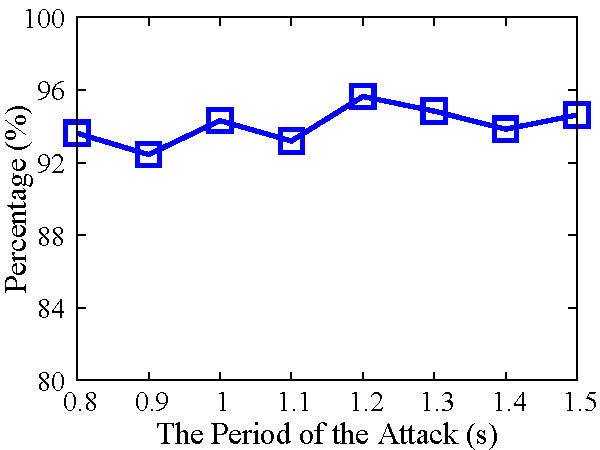
\includegraphics[scale=0.7]{recall}
%         \caption{\small{识别单攻击源LDoS召回率}}
%         \label{fig:recall}
%     \end{minipage}
%     \begin{minipage}[t]{0.49\linewidth}
%         \centering
%         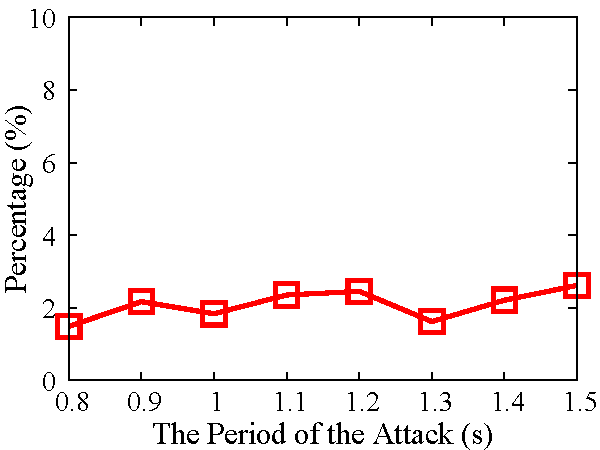
\includegraphics[scale=0.7]{false_positive}
%         \caption{\small{识别单攻击源LDoS误判率}}
%         \label{fig:false_positive1}
%     \end{minipage}
% \end{figure}

\begin{figure}
    \begin{subfigure}{.49\textwidth}
        \centering
        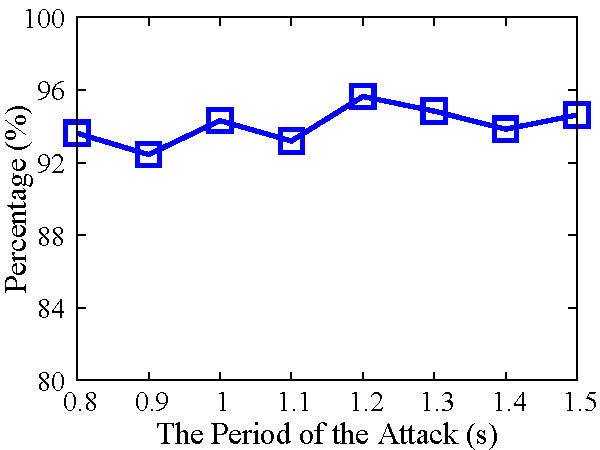
\includegraphics[scale=0.7]{recall}
        \caption{召回率}
        \label{fig:recall}
    \end{subfigure}
    \begin{subfigure}{.49\textwidth}
        \centering
        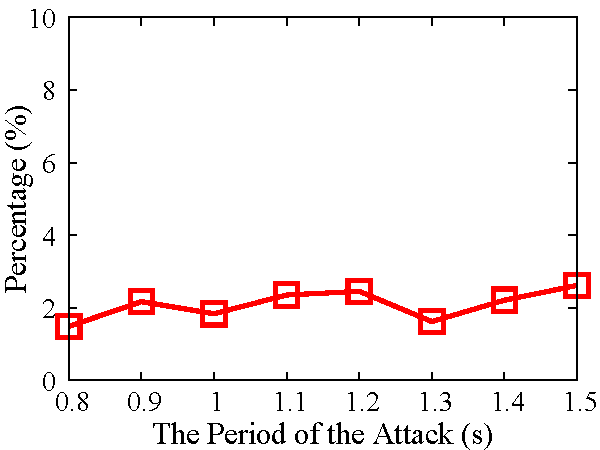
\includegraphics[scale=0.7]{false_positive}
        \caption{误判率}
        \label{fig:false-positive}
    \end{subfigure}
    \caption{识别单攻击源LDoS攻击}
    \label{fig:accuracy-single}
\end{figure}

首先是单攻击源LDoS攻击召回率与误判率。经过多次实验测量,单攻击源召回率相对如图\ref{fig:recall}所示,不管LDoS攻击的$T$和$L$如何变化,识别率在92\%至96\%之间,最低的识别率都高于90\%,这表明攻击定位模块能够确定大多数的单攻击源LDoS攻击流,使用平均欧式距离方法来判断LDoS攻击流是一种非常有效的方法。但是系统也存在一定的误判率,如图\ref{fig:false-positive}所示,正常流被误判成为LDoS攻击流的情况也是存在的,但是误判率较低,最高也不超过5\%,大部分的LDoS流对绝大多数的正常流都不会有影响。


\begin{figure}
    \begin{subfigure}{.49\textwidth}
        \centering
        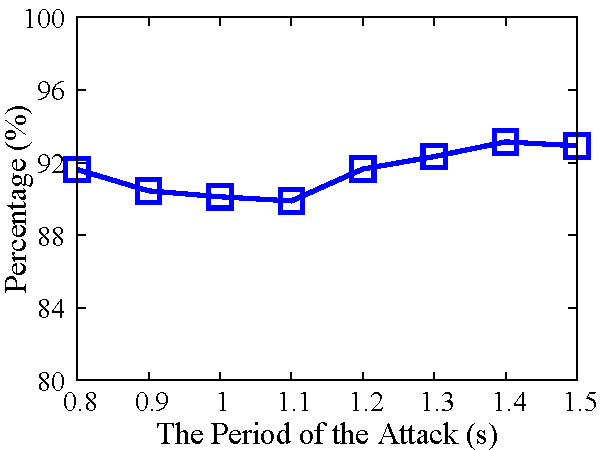
\includegraphics[scale=0.7]{recall1}
        \caption{召回率}
        \label{fig:recall1}
    \end{subfigure}
    \begin{subfigure}{.49\textwidth}
        \centering
        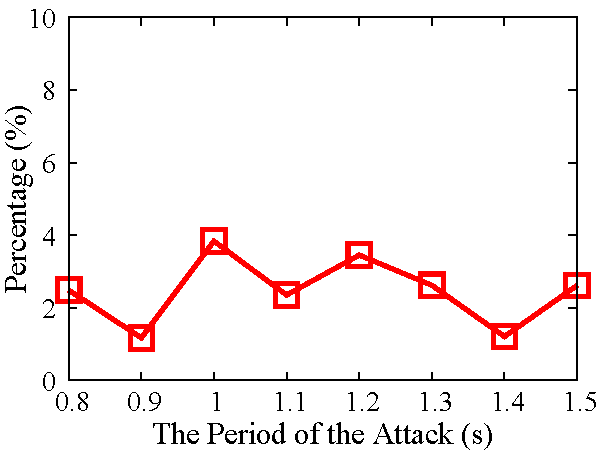
\includegraphics[scale=0.7]{false_positive1}
        \caption{误判率}
        \label{fig:false-positive1}
    \end{subfigure}
    \caption{分布式方案一的LDoS攻击}
    \label{fig:accuracy-2h-mod1}
\end{figure}

接下来,讨论分布式方案一的LDoS攻击的召回率和误判率。如图\ref{fig:recall1}攻击定位模块识别分布式方案一的LDoS攻击的召回率基本上在90\%至94\%之间,但是与单攻击源对比,召回率是有所下降的。这说明以分布式方案一的LDoS攻击比起单攻击源的LDoS攻击有更加强的隐蔽性,不过,攻击定位模块对分布式方案一的LDoS攻击召回率还是很高,最低的召回率为89.8\%。攻击定位模块的误判率也不高,如图\ref{fig:false-positive1}所示,最高误判率也不超过5\%。这样的结果与单攻击源的LDoS的误判率类似,说明不管LDoS攻击以何种方式来生成的都不影响攻击定位模块对正常流的判断。

\begin{figure}
    \begin{subfigure}{.49\textwidth}
        \centering
        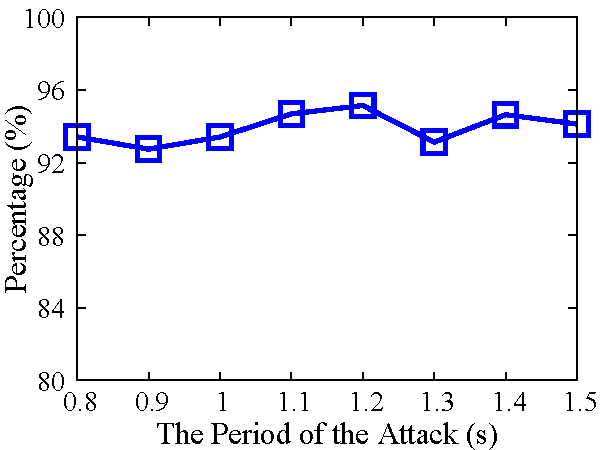
\includegraphics[scale=0.7]{recall2}
        \caption{召回率}
        \label{fig:recall2}
    \end{subfigure}
    \begin{subfigure}{.49\textwidth}
        \centering
        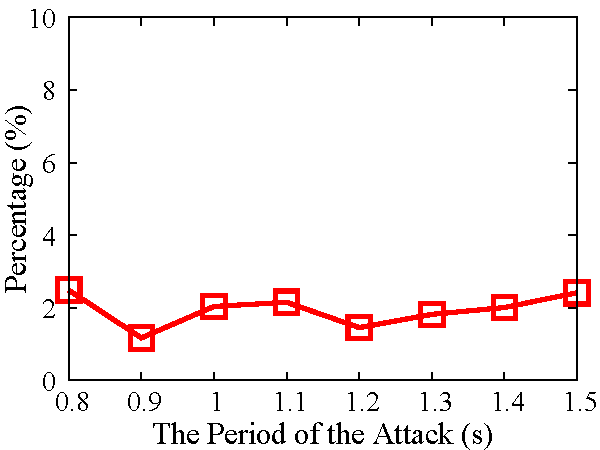
\includegraphics[scale=0.7]{false_positive2}
        \caption{误判率}
        \label{fig:false-positive2}
    \end{subfigure}
    \caption{分布式方案二的LDoS攻击}
    \label{fig:accuracy-2h-mod2}
\end{figure}

\begin{figure}
    \begin{subfigure}{.49\textwidth}
        \centering
        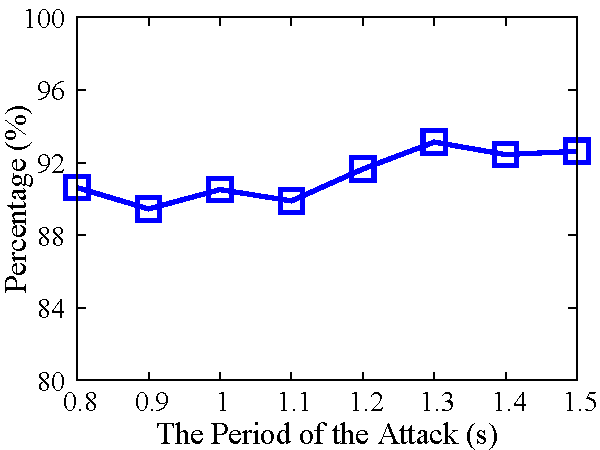
\includegraphics[scale=0.7]{recall3}
        \caption{召回率}
        \label{fig:recall3}
    \end{subfigure}
    \begin{subfigure}{.49\textwidth}
        \centering
        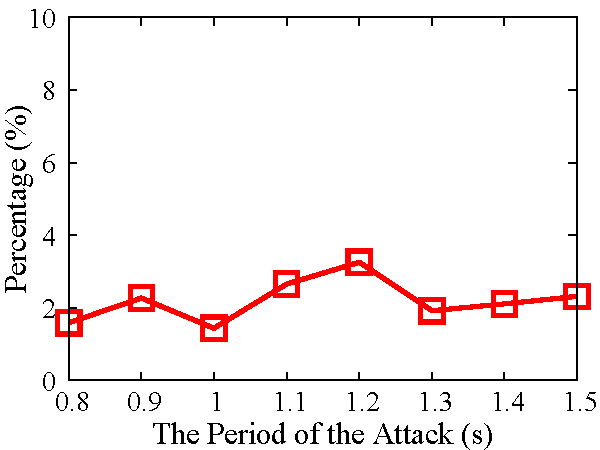
\includegraphics[scale=0.7]{false_positive3}
        \caption{误判率}
        \label{fig:false-positive3}
    \end{subfigure}
    \caption{分布式方案三的LDoS攻击}
    \label{fig:accuracy-2h-mod3}
\end{figure}

如图\ref{fig:recall2}所示,当LDoS攻击以分布式方案二生成LDoS攻击流量的时候,使用攻击定位模块识别LDoS攻击的召回率在92\%至95\%之间。相较于分布式方案一,分布式方案二的召回率更高,这说明减小LDoS攻击的峰值速率对于攻击定位模块识别LDoS攻击流的影响不大。分布式方案二的召回率与单攻击源的召回率接近,是因为,分布式方案二的LDoS攻击流的二值化序列的形状与单攻击源相同。此时,攻击定位模块的误判率如图\ref{fig:false-positive2}所示,不管是LDoS攻击的$L$与$T$如何变化,误判率都低于5\%,与前两种方案的结果相似。

最后,分析LDoS攻击以分布式方案三生成LDoS攻击流量的情况。如图\ref{fig:recall3}所示,使用攻击定位模块识别LDoS攻击流,召回率在89\%至93\%之间,比单攻击源的召回率更低,与分布式方案一接近,这说明分布式方案三也具备一定的隐蔽性,但是,攻击定位模块的最低识别率是89.4\%,供给定位模块识别LDoS攻击流的效果还是很好的。而误判率的情况如图\ref{fig:recall3}所示,误判率低于5\%。大部分情况下,正常流被误判为攻击流的情况是很难出现的。

综上所述,分布式方案一与分布式方案三的LDoS攻击流相对于单攻击源和分布式方案二的LDoS攻击流具有更加好的隐蔽性,所以攻击定位模块在识别分布式方案一与分布式方案三的LDoS攻击流的召回率比识别单攻击源和分布式方案二的LDoS攻击流的要更低。因为在每个$T$中,使用分布式方案一与分布式方案三的LDoS攻击流的平均突发时间长度为持续$L/2$,而单攻击源和分布式方案二的LDoS攻击流的平均突发事件长度为$L$。LDoS攻击流是单攻击源还是分布式都不影响攻击定位模块对于正常流的误判率,因为只要LDoS攻击的$T$和$L$确定了,在端口上汇聚的LDoS攻击流的二值序列就确定了,对正常流造成的效果也是一样的。


\subsection{防御方案评价}
\label{chap05:evaluaion}

这一部分的主要的内容是评价防御方案的有效性和使用方案的系统开销。为了验证防御方案的有效性,本文对比在部署防御系统与没有防御系统的两种条件下,LDoS攻击存在时的TCP流的吞吐量。然后,为了获取方案的系统开销。在部署防御系统的情况下,通过生成不同$T$的LDoS攻击来测试控制器的CPU使用率。

为了验证有效性,本文测试有无防御系统的条件下,LDoS攻击存在时的TCP流的吞吐量。在系统
生成了100个TCP攻击流,并让这些流经过同一个端口。与此同时,通过攻击主机以单攻击源和分布式方案等四种方式发送LDoS攻击流量($T$为210毫秒,$L$为90毫秒,$R$为1Gbps)经过该端口,同时也注入背景流量。在防御方案使用流表规则阻塞LDoS攻击的情况下,进行测试。图\ref{fig:throughput-single}为在单攻击源LDoS攻击流下TCP流的聚合吞吐量。实验记录了30秒的TCP流聚合吞吐量。从图中可以看出,在没有防御系统防御LDoS攻击流的时候,TCP流的聚合吞吐量平均值只有5Mbps。当有了防御系统之后,LDoS攻击能够在入口交换机出被流表规则阻塞。因此,在部署了防御系统之后,TCP流的聚合吞吐量的平均值上升至580Mbps。在LDoS攻击的影响下,TCP流的聚合吞吐量下降到很低的程度,是因为LDoS攻击迫使一些TCP流进入了超时重传状态。这也能证明SDN中基于动态周期性检测的LDoS防御方案能够有效的限制LDoS攻击。

\begin{figure}
    \begin{subfigure}{.49\textwidth}
        \centering
        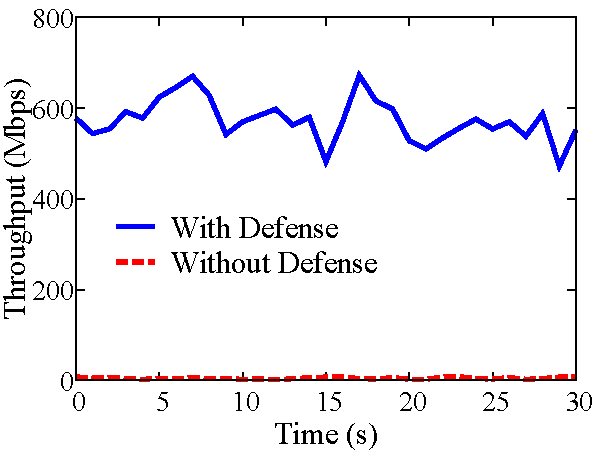
\includegraphics[scale=0.7]{throughput}
        \caption{单攻击源}
        \label{fig:throughput-single}
    \end{subfigure}
    \begin{subfigure}{.49\textwidth}
        \centering
        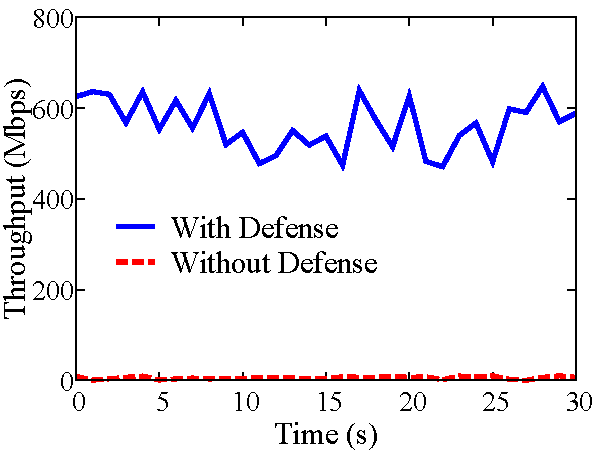
\includegraphics[scale=0.7]{throughput1}
        \caption{分布式方案一}
        \label{fig:throughput-2h-mod1}
    \end{subfigure}

    \begin{subfigure}{.49\textwidth}
        \centering
        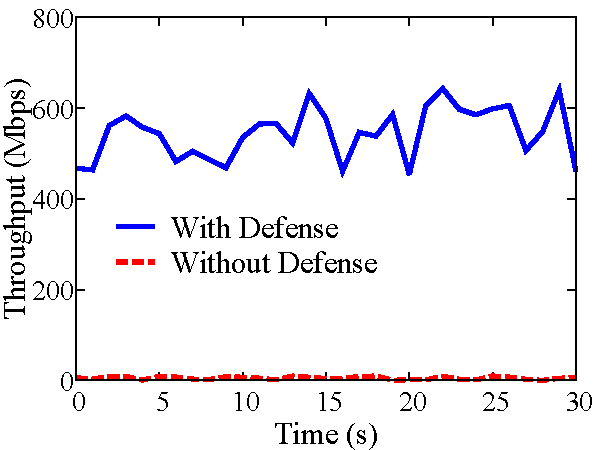
\includegraphics[scale=0.7]{throughput2}
        \caption{分布式方案二}
        \label{fig:throughput-2h-mod2}
    \end{subfigure}
    \begin{subfigure}{.49\textwidth}
        \centering
        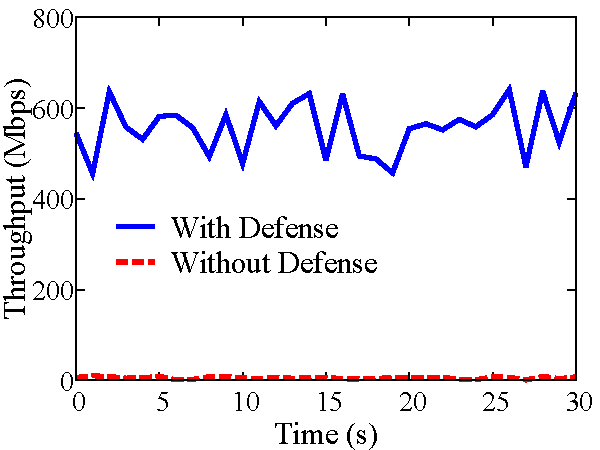
\includegraphics[scale=0.7]{throughput3}
        \caption{分布式方案三}
        \label{fig:throughput-2h-mod3}
    \end{subfigure}


    \caption{使用流表规则阻塞LDoS攻击的TCP流聚合吞吐量}
    \label{fig:throughput-all}
\end{figure}

图\ref{fig:throughput-2h-mod1}是在分布式方案一生成LDoS攻击下的TCP流聚合吞吐量。通过两个主机的协同发送LDoS攻击,在受影响端口处形成LDoS攻击流量。在没有防御系统的时候,TCP流的聚合吞吐量平均值为6Mbps。在有防御系统之后,TCP流的聚合吞吐量平均值上升至接近600Mbps的程度。这说明,分布式方案一的LDoS攻击流能够达到单攻击源的攻击效果,迫使TCP流不断进入超时重传状态。在部署防御方案之后,吞吐量恢复正常,这说明防御系统对分布式方案一生成的LDoS攻击流也是有效的,分布式LDoS攻击也被流表规则在入口交换机处阻塞。

图\ref{fig:throughput-2h-mod2}是在分布式方案二生成LDoS攻击流下的TCP流聚合吞吐量。两个主机降低峰值速率至500Mbps,计算好时延,发送的LDoS攻击流量在受影响端口处汇聚。在没有防御系统的时候,TCP流的聚合吞吐量平均值为4Mbps。这说明,分布式方案二是有效的分布式LDoS攻击方案,它能迫使TCP流不断进入超时重传状态。但是在防御系统的保护下,TCP流的聚合吞吐量平均值超过550Mbps。这说明防御系统能够有效的防御分布式方案二生成的LDoS攻击流,流表规则在入口交换机处阻塞了分布式方案二生成的LDoS攻击。

图\ref{fig:throughput-2h-mod3}是以分布式方案三生成LDoS攻击流量的TCP流聚合吞吐量。在两个主机协同发送数据流,两个书籍在每个突发都发送$L/2$的LDoS攻击流先后到达受影响端口。在没有防御系统的时候,TCP流的聚合吞吐量平均值为5Mbps。这说明,分布式方案三是有效地能迫使TCP流不断进入超时重传状态。但是在防御系统的保护下,TCP流的聚合吞吐量平均值提升至400Mbps以上的速率。这说明分布式方案三生成的LDoS攻击流依然被防御系统限制,安装在入口交换机处的流表规则阻塞了分布式方案三生成的LDoS攻击。

在图\ref{fig:throughput-all}中的四个图证明了防御方案对四种形式的LDoS攻击都是有效的,防御系统能够通过防御方案定位攻击源并安装限制的流表规则阻塞LDoS攻击流,最大程度的减小了LDoS攻击对系统的影响。


\begin{figure}
    \begin{subfigure}{.49\textwidth}
        \centering
        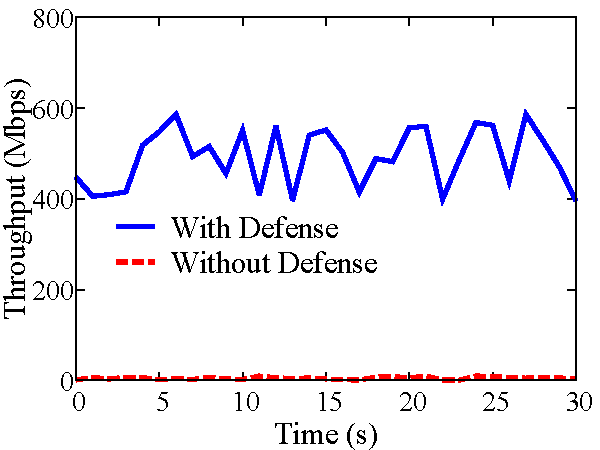
\includegraphics[scale=0.7]{meterthroughput}
        \caption{单攻击源}
        \label{fig:meter-throughput-single}
    \end{subfigure}
    \begin{subfigure}{.49\textwidth}
        \centering
        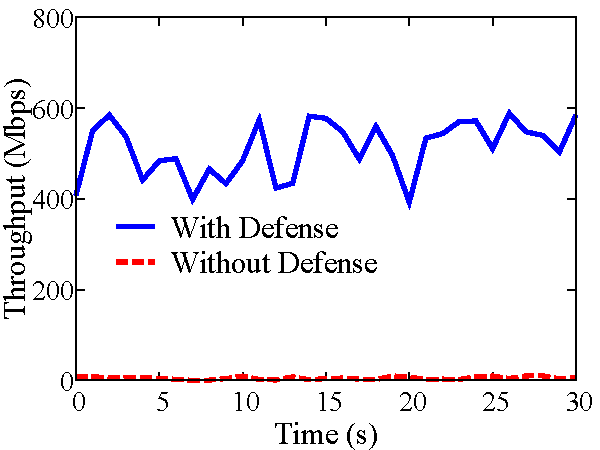
\includegraphics[scale=0.7]{meterthroughput1}
        \caption{分布式方案一}
        \label{fig:meter-throughput-2h-mod1}
    \end{subfigure}

    \begin{subfigure}{.49\textwidth}
        \centering
        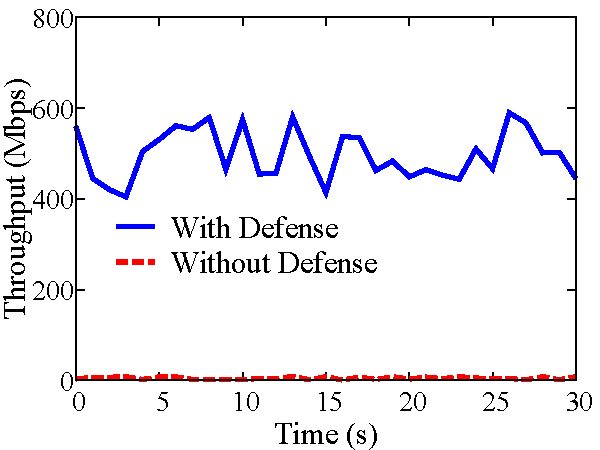
\includegraphics[scale=0.7]{meterthroughput2}
        \caption{分布式方案二}
        \label{fig:meter-throughput-2h-mod2}
    \end{subfigure}
    \begin{subfigure}{.49\textwidth}
        \centering
        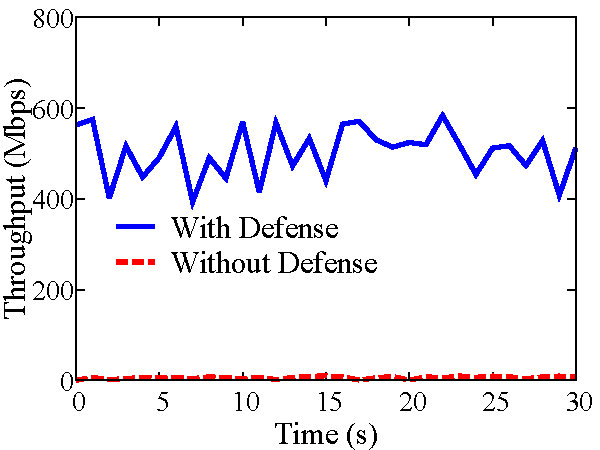
\includegraphics[scale=0.7]{meterthroughput3}
        \caption{分布式方案三}
        \label{fig:meter-throughput-2h-mod3}
    \end{subfigure}


    \caption{使用Meter规则限制LDoS攻击的TCP流聚合吞吐量}
    \label{fig:meter-throughput-all}
\end{figure}


在防御方案使用Meter规则限制LDoS攻击的情况下,进行测试。在防御系统确认一个流为LDoS攻击流的时候,使用特制的Meter规则对LDoS攻击流的速率限制。在实验中,限制被识别的LDoS攻击流的速率为100Mbps。则在之前的实验环境在再进行一次测试,则可验证方案使用Meter规则限制LDoS攻击方法的有效性。图\ref{fig:meter-throughput-single}为单攻击源的LDoS攻击流下TCP流的聚合吞吐量。实验同样也是记录30秒内的TCP流的聚合吞吐量。在防御系统的保护下,TCP流聚合吞吐量的平均值为500Mbps,比使用流表规则对LDoS攻击源进行阻塞的平均值要更低,因为,限制LDoS攻击流依然使用部分带宽。没有防御的时候,TCP流的聚合吞吐量平均数不超过10Mbps。证明了使用Meter规则限制LDoS攻击的方案是可行的。

图\ref{fig:meter-throughput-2h-mod1}为分布式方案一的LDoS攻击流下TCP流的聚合吞吐量。图\ref{fig:meter-throughput-2h-mod2}分布式方案二的LDoS攻击流下TCP流的聚合吞吐量。图\ref{fig:meter-throughput-2h-mod3}分布式方案三的LDoS攻击流下TCP流的聚合吞吐量。通过三个图可以看出,使用Meter规则能够限制分布式LDoS攻击。效果与单攻击源一致,这证明防御系统已经找到了所有的攻击源并限制LDoS流量。但是,吞吐量都相较于使用流表规则对LDoS攻击源进行阻塞更低。

从图\ref{fig:throughput-all}和图\ref{fig:meter-throughput-all}可以看出,不管是使用流表规则阻塞LDoS攻击,还是使用Meter规则限制LDoS攻击的速率都能够使TCP流避免由于丢包而进入超时重传状态,保证了TCP流的正常传输。但是,两种方式各有优劣。使用流表规则阻塞LDoS攻击流,避免LDoS攻击流进入系统带来安全的隐患,同时,还能给TCP流提供更多的带宽,不过也有流因为被误判为攻击流而无法进行正常的传输。同时,通过测试,使用Meter规则限制LDoS攻击同样是有效的,但是,由于保留了LDoS攻击流的部分带宽,TCP流的可用带宽也减少了很多。

在控制器上部署了防御系统后,系统在检测和限制各种LDoS攻击的系统开销是评价系统很重要的一个指标。通过对比有防御系统和没有防御系统的系统开销。在实验中,将LDoS攻击$T$由0.1秒逐步提升至1秒,同时也测试了洪泛攻击。图\ref{fig:CPU-single}展示了防御系统限制单攻击源的LDoS攻击流的系统开销。控制器的开销随着LDoS攻击的$T$减小而增大。更小的$T$的LDoS攻击给控制器造成的系统开销越大。因为随着LDoS攻击的$T$减小,根据奈奎斯特准则,控制器需要减小采样间隔$T_b$才能计算出LDoS攻击的$T$,因此,控制器需要处理的序列长度更长,引入的开销更大。一般情况下,LDoS攻击的$T$都会大于0.2s,所以,防御系统在大多数时候给系统引入的额外开销低于2\%。

\begin{figure}
    \begin{subfigure}{.49\textwidth}
        \centering
        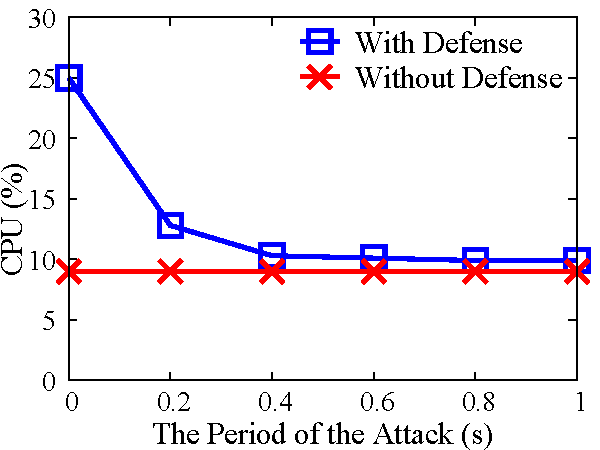
\includegraphics[scale=0.7]{utilization}
        \caption{单攻击源}
        \label{fig:CPU-single}
    \end{subfigure}
    \begin{subfigure}{.49\textwidth}
        \centering
        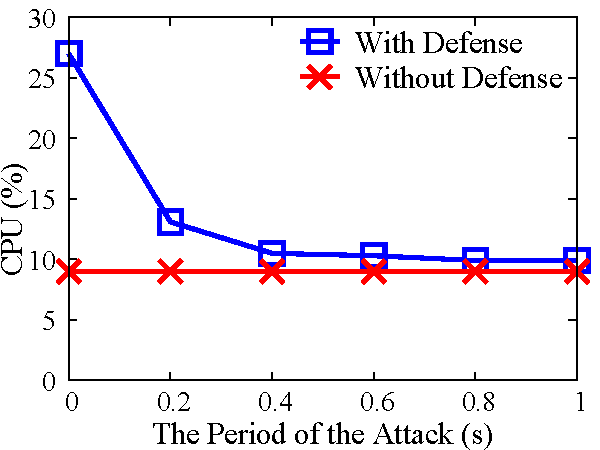
\includegraphics[scale=0.7]{utilization1}
        \caption{分布式方案一}
        \label{fig:CPU-2h-mod1}
    \end{subfigure}

    \begin{subfigure}{.49\textwidth}
        \centering
        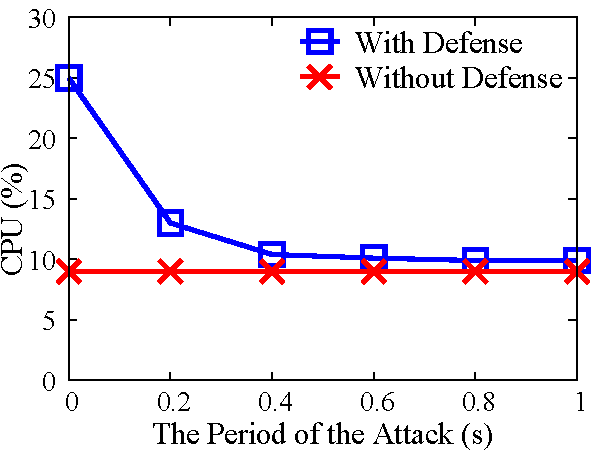
\includegraphics[scale=0.7]{utilization2}
        \caption{分布式方案二}
        \label{fig:CPU-2h-mod2}
    \end{subfigure}
    \begin{subfigure}{.49\textwidth}
        \centering
        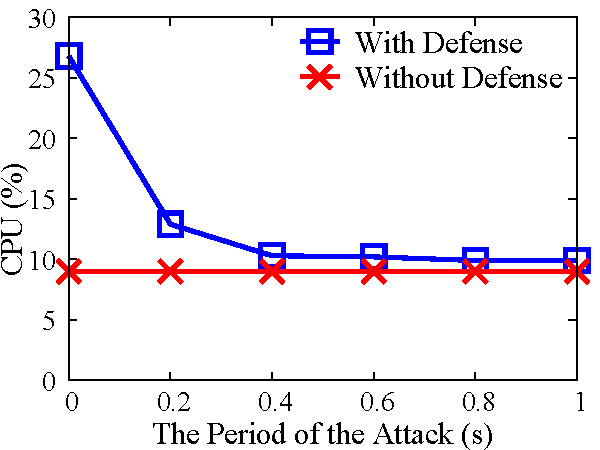
\includegraphics[scale=0.7]{utilization3}
        \caption{分布式方案三}
        \label{fig:CPU-2h-mod3}
    \end{subfigure}


    \caption{CPU使用率}
    \label{fig:CPU-all}
\end{figure}

图\ref{fig:CPU-2h-mod1}为展示了防御系统限制以分布式方案一的生成LDoS攻击流的系统开销。
图\ref{fig:CPU-2h-mod2}为展示了防御系统限制以分布式方案二的生成LDoS攻击流的系统开销。
图\ref{fig:CPU-2h-mod3}为展示了防御系统限制以分布式方案三的生成LDoS攻击流的系统开销。从这三个图可以看出,在防御分布式LDoS攻击的时候,控制器的开销同样随着LDoS攻击的$T$减小而增大。更小的$T$的LDoS攻击引入的控制器开销越大。原因与单攻击源相同,使用更小的$T_b$才能计算出LDoS攻击的$T$。防御系统在大多数情况下引入的系统额外开销低于2\%。

综上所述,系统的开销只与LDoS攻击的$T$相关,与LDoS攻击是单攻击源还是分布式无关。因为,系统的主要开销在计算异常端口的周期上,所以,LDoS攻击的$T$越小,引入的系统开销越大。不过,大部分情况下,系统引入的额外开销都低于2\%,这样的开销对于部署基于动态周期性检测的LDoS防御方案是可以接受的。


\section{两方案比较}
\label{chap05:compare}

基于带宽保障的方案和基于动态周期性检测的方案在限制LDoS攻击的